\documentclass{article} % For LaTeX2e
\usepackage{iclr2015,times}
\usepackage{hyperref}
\usepackage{url}

\usepackage{array}
\usepackage{subfigure}
\usepackage{epsfig}
\usepackage{graphicx}
\usepackage{amsmath}
\usepackage{amssymb}
\usepackage{bbm}
\usepackage{epstopdf}
\usepackage{caption}
%\usepackage{subcaption}
\usepackage{enumitem}
\usepackage{calc}
\usepackage{multirow}
\usepackage{xspace}

\newcommand{\figref}[1]{Fig\onedot~\ref{#1}}
\newcommand{\equref}[1]{Eq\onedot~\eqref{#1}}
\newcommand{\secref}[1]{Sec\onedot~\ref{#1}}
\newcommand{\tabref}[1]{Tab\onedot~\ref{#1}}
\newcommand{\thmref}[1]{Theorem~\ref{#1}}
\newcommand{\prgref}[1]{Program~\ref{#1}}
\newcommand{\algref}[1]{Alg\onedot~\ref{#1}}
\newcommand{\clmref}[1]{Claim~\ref{#1}}
\newcommand{\lemref}[1]{Lemma~\ref{#1}}
\newcommand{\ptyref}[1]{Property\onedot~\ref{#1}}

\newcommand{\by}[2]{\ensuremath{#1 \! \times \! #2}}

\makeatletter 
\DeclareRobustCommand\onedot{\futurelet\@let@token\@onedot}
\def\@onedot{\ifx\@let@token.\else.\null\fi\xspace}
\def\eg{\emph{e.g}\onedot} \def\Eg{\emph{E.g}\onedot}
\def\ie{\emph{i.e}\onedot} \def\Ie{\emph{I.e}\onedot}
\def\cf{\emph{cf}\onedot} \def\Cf{\emph{Cf}\onedot}
\def\etc{\emph{etc}\onedot} \def\vs{\emph{vs}\onedot}
\def\wrt{w.r.t\onedot} \def\dof{d.o.f\onedot}
\def\etal{\emph{et al}\onedot}

%%%%%%%%%%%%%%%%%%%%%%%%%%%%%%%%%%%%%%%%
\title{Semantic Image Labeling with Deep Convolutional Networks and Fully Connected CRFs}

\author{
Liang-Chieh Chen\\
Univ\onedot of California, Los Angeles\\
\texttt{lcchen@cs.ucla.edu}
\And
George Papandreou \thanks{Work performed while G.P\onedot was with the Toyota
  Technological Institute at Chicago. The first two authors contributed
  equally to this work.}\\
Google Inc.\\
\texttt{gpapan@google.com}\\
\And
Iasonas Kokkinos\\
\'Ecole Centrale Paris and INRIA\\
\texttt{iasonas.kokkinos@ecp.fr}\\
\And
Kevin Murphy\\
Google Inc.\\
\texttt{kpmurphy@google.com}\\
\And
Alan L. Yuille\\
Univ\onedot of California, Los Angeles\\
\texttt{yuille@stat.ucla.edu} 
}

% The \author macro works with any number of authors. There are two commands
% used to separate the names and addresses of multiple authors: \And and \AND.
%
% Using \And between authors leaves it to \LaTeX{} to determine where to break
% the lines. Using \AND forces a linebreak at that point. So, if \LaTeX{}
% puts 3 of 4 authors names on the first line, and the last on the second
% line, try using \AND instead of \And before the third author name.

\newcommand{\fix}{\marginpar{FIX}}
\newcommand{\new}{\marginpar{NEW}}

%\iclrfinalcopy % Uncomment for camera-ready version

\iclrconference % Uncomment if submitted as conference paper instead of workshop

\begin{document}


\maketitle


%%%%%%%%% ABSTRACT
\newcommand{\mycomment}[1]{}
\begin{abstract}
 Deep Convolutional Neural Networks (DCNN) have decisevely pushed the envelope of  high-level vision over the last couple of years, but their applications to low-level tasks are often still not up the level of  computer vision systems using simple classifiers with well-engineered features. Our understanding is that this can be due to the increased invariance of DCNNs to local image transformations, and in this work we aim at  accommodating the effects of this invariance in the context of semantic segmetnation.

Our main contribution consists in  increasing the spatial acuity of DCNNs  by combining their invariant classification results with bottom-up, image-driven cues for segmentation. 
In particular, we first demonstrate that simple modifications to the standard architectures used for object classification can deliver impessively accurate semantic segmentation results while operating at XXX frames-per-seconds. More importantly, we couple DCNNs  with Mean Field inference for Markov Random Fields  and obtain state-of-the-art results on the PASCAL semantic image segmentation task.  

\mycomment{We consider our main contribution to be the increase of the acuity of DCNNs, by combining invariant classifications with bottom-up, image-driven cues for segmentation.} 
\end{abstract}



%%%%%%%%% BODY TEXT
\section{Introduction}
\label{sec:intro}
%established in machine learning 
Deep Convolutional Neural Networks (DCNNs) had been the method of choice for document recognition since  \citet{LeCun1998}, but 
have only recently become the mainstream of high-level vision research.
Over the past two years  DCNNs have pushed the performance of computer vision systems to soaring heights on a broad array of high-level problems, including image classification \citet{KrizhevskyNIPS2013, papandreou2014untangling, sermanet2013overfeat, simonyan2014very, szegedy2014going}, object detection \citet{girshick2014rcnn}, fine-grained categorization \citet{zhang2014part} and pose estimation \citet{chen2014articulated, tompson2014joint}, among others.
The most consistent result in these works is that DCNNs trained in an end-to-end manner  deliver  strikingly better results than systems relying on carefully engineered features, such as SIFT or HOG features.
This success can be partially attributed to the built-in  invariance of DCNNs to local image transformations, which underpins their ability to learn hierarchical abstractions of data \citep{zeiler2014visualizing}. While this invariance is clearly desirable for high-level vision tasks, it can hamper low-level tasks, such as semantic segmentation - where we want precise localization, rather than abstraction of spatial details.  As such, the DCNN architectures leading the game of high-level vision are not yet exploitable `out of the box' for low-level vision tasks, such as dense image labelling. 


%However, the applications of DCNNs to low-level vision tasks, such as segmentation, or semantic image labelling still lags a bit behind in performance, with existing DCNN systems underpeforming  systems that use flat classifiers with well-engineered features, as witnessed e.g. in boundary detection with DCNNs \cite{williams14} as opposed to the  Forest-based system of \cite{DollarZ13}. 

There are two technical hurdles in the application of DCNNs to image labelling
tasks: signal downsampling, and spatial `insensitivity' (invariance).  The
first problem relates to the reduction of signal resolution incurred by the
repeated combination of max-pooling and downsampling (`striding') performed at
every layer of standard DCNNs, e.g. \citep{KrizhevskyNIPS2013,
  simonyan2014very, szegedy2014going}. Instead, as in
\cite{papandreou2014untangling}, we introduce into the problem the `atrous'
(with holes) algorithm originally developed for efficiently computing the
discrete wavelet transform \cite{Mall99}, thereby achieving substantial gains
in efficiency over this naive approach.

The second problem relates to the fact that obtaining object-centric decisions
from a classifier inherently requires invariance to spatial
transformations. For instance, we cannot expect a `bicycle' classifier to
respond differently to pixels that are placed on the bicycle's support and to
pixels that are placed in the interior of its holes, e.g. within the bicycle's
chassis, or rays. In order to deal with this problem we turn to Conditional
Random Fields (CRFs) that have been broadly used in semantic segmentation to
combine class scores computed by multi-way classifiers with the low-level
information captured by the local interactions of pixels and edges
\citep{rother2004grabcut, shotton2009textonboost} or superpixels
\citep{lucchi2011spatial}. Even though works of increased sophistication have
been proposed to model the hierarchical dependency \citep{he2004multiscale,
  ladicky2009associative, lempitsky2011pylon} and/or high-order dependencies
of segments \citep{delong2012fast, gonfaus2010harmony, kohli2009robust}, we
use the fully connected pairwise CRF proposed by
\citet{krahenbuhl2011efficient} for its efficient computation, and ability to
capture long range dependencies. That model was shown in
\citet{krahenbuhl2011efficient} to largely improve the performance of a
boosting-based pixel-level classifier, and in our work we demonstrate that it
leads to state-of-the-art results when coupled with a DCNN-based pixel-level
classifier.

%invariance that is inherently necessary in order to obtain high-level, 
%In brief, we treat the first side of the problem by , and the second by coupling DCNNs with Conditional Random Field inference, so as to combine the high-level decisons of DCNNs with the sharp spatial localization of CRFs.

There  three main advantages of our method are (i) speed: by virtue of the `atrous' algorithm our DCNN classifier operates at 8 fps, while Mean Field Inference for the fully-connected CRF requires 0.5 second, (ii) accuracy: we obtain state-of-the-art results on the PASCAL semantic segmentation challenge, outperforming the second-best approach of \citet{mostajabi2014feedforward} by a factor of 2$\%$ and (iii) simplicity: our system is composed of a cascade of two fairly well-established modules, DCNNs and CRFs, that can eventually be jointly trained with backpropagation. 

%In particular, when compared to a broad pool of works recently developped around the problem of combining DCNNs with semantic segmentation, our system can be understood as being substantially simpler, relying on a minimal number of components, while at the same time delivering state-of-the-art results.

%\citet{mostajabi2014feedforward} 

This is in contrast to the two-stage approaches that are now most common in semantic segmentation with DCNNs: such techniques typically use a cascade of bottom-up image segmentation and DCNN-based region classification, which makes the system commit to whatever errors of the front-end segmentation system.  
For instance, the bounding box proposals and masked regions delivered by \citep{arbelaez2014multiscale, Uijlings13} are used in 
\citet{girshick2014rcnn} and \cite{hariharan2014simultaneous}  as inputs to a DCNN to introduce  shape information into the classification process. Similarly, the authors of  \citet{mostajabi2014feedforward} label pre-computed superpixels using multi-scale DCNN cues extracted around them with some hand-crafted features, while a celebrated  non-DCNN precursor to these  works
is the second order pooling method of \citep{carreira2012semantic} which also assigns labels to the regions proposals delivered by \citep{carreira2012cpmc}. 
Understanding the perils of committing to a single segmentation, the authors of \citet{cogswell2014combining} 
build on \citep{yadollahpour2013discriminative} to explore a diverse set of CRF-based segmentation proposals, computed also by \citep{carreira2012cpmc}. These segmentation proposals are then re-ranked according to a DCNN trained in  particular for this reranking task. Even though this approach explicitly tries to handle the temperamental nature of a front-end segmentation algorithm, there is still no explicit exploitation of the DCNN scores in  the CRF-based segmentation algorithm: the DCNN is only applied post-hoc, while it would make sense to directly try to use its results {\em during} segmentation. 
% and the DCNN

Moving towards works that lie closer to our approach, several other researchers have considered the use of convolutionally computed DCNN features for dense image labelling -potentially coupled with some segmentation post-processing, rather than pre-processing. Among the first have been
\citet{farabet2013learning} who apply DCNNs at multiple image resolutions and then employ a segmentation tree to smooth the prediction results; more recently, \citet{hariharan2014hypercolumns} propose to concatenate the computed inter-mediate feature maps within the DCNNs for pixel classification, and \citet{dai2014convolutional} propose to pool the inter-mediate feature maps by region proposals. Even though these works still employ  segmentation algorithms that are  decoupled from the DCNN classifier's results, we believe it is advantageous that segmentation is only used at a later stage, avoiding the commitment  to premature decisions. 

%, but also  heavily depends on the region proposals;  a similar approach using manually engineered features is 
%. We also notice that there are serveral concurrent works, which bear similarities to our proposed model.  However, they results depend on the superpixels, which may leak out the object boundaries.  Their models are two-step models, which depends on the accuracy of first step (\ie region proposals). 

More recently, the segmentation-free techniques of \citet{long2014fully} and \cite{eigen2014predicting} directly apply DCNNs to the whole image in a sliding window fashion, replacing the last fully connected layers of a DCNN  by convolutional layers. In order to deal with the spatial localization issues outlined in the beginning of the introduction, \citet{long2014fully} upsample and concatenate the scores from inter-mediate feature maps, while \citet{eigen2014predicting} refine the prediction result from coarse to fine by propagating the coarse results to another DCNN. 

%Another recent work that also attempts to combine the effectiveness of graphical model and DCNNs for segmentation is \citet{cogswell2014combining}, where the authors employ CRFs to propose diverse region proposals, an extension of \citet{yadollahpour2013discriminative}.

The main difference between our model and other state-of-the-art models is the combination of pixel-level CRFs and DCNN-based `unary terms'. Focusing on the closest    works in this direction, we remind  that  the authors of \citet{cogswell2014combining} use CRFs as a proposal mechanism for a DCNN-based reranking system, while the authors of  
\citet{farabet2013learning} treat superpixels as  nodes for a local pairwise CRF and use graph-cuts for discrete inference; as such their results can be limited by errors in superpixel computations, while ignoring  long-range superpixel dependencies. Our approach instead treats every pixel as a CRF node, exploits long-range dependencies, and uses  CRF inference to directly optimize a DCNN-driven cost function. 

% used in our fully-connected CRF. 
 %extract features via DCNN
%the one is by , who
% also employ CRF to propose diverse region proposals , and \citet{chen2014learning} which efficiently blend inference and learning to jointly train DCNN and CRF. 
%Our current model employs piecewise training, and jointly training is our next goal.


%{\bf{Conditional Random Fields for segmentation
%,  or crop several  bounding boxes from an image \citep{, girshick2014rcnn} to deal with multiple objects.


%: %}} Many semantic segmentation methods rely on Conditional Random Fields (CRFs), which

%{\bf{Deep Convolutional Neural Network for segmentation: }} Most of the systems built on top of DCNNs classify either a single object label for an entire image \citep{KrizhevskyNIPS2013, simonyan2014very, szegedy2014going}, or several object labels for bounding boxes within an image \citep{papandreou2014untangling, girshick2014rcnn}. Recently, there are several works that attemp to semantically segment an image with DCNNs. 




%\subsection{Related Work}
Our model is mostly related to two fields, and the goal of this work is to combine the best from them.

{\bf{Conditional Random Fields for segmentation: }} Many semantic segmentation methods rely on Conditional Random Fields (CRFs), which model the local interactions between pixels \citep{rother2004grabcut, shotton2009textonboost} or superpixels \citep{lucchi2011spatial} via the pairwise potential. Several works have been proposed to model the hierarchical dependency \citep{he2004multiscale, ladicky2009associative, lempitsky2011pylon} and the high-order potential (in addition to pairwise potential) \citep{delong2012fast, gonfaus2010harmony, kohli2009robust, krahenbuhl2011efficient}. Our model takes use of the efficient inference algorithm in fully connected CRF proposed by \citet{krahenbuhl2011efficient} for its powerful long range dependency.

{\bf{Deep Convolutional Neural Network for segmentation: }} Most of the systems built on top of DCNN classify either a single object label for an entire image \citep{KrizhevskyNIPS2013, simonyan2014very, szegedy2014going}, or several object labels for bounding boxes within an image \citep{papandreou2014untangling, girshick2014rcnn}. Recently, there are several works that attemp to semantically segment an image with DCNN. \citet{girshick2014rcnn, hariharan2014simultaneous} take both bounding box proposals and masked regions as input to DCNN. The masked regions provide extra object shape informantion to the neural networks. These methods heavily depend on the region proposals \citep{arbelaez2014multiscale, Uijlings13}. 
%Note that second order pooling \citep{carreira2012semantic} also assigns labels to regions proposals \citep{carreira2012cpmc}; however, hand-crafted features are employed. 
\citet{farabet2013learning} apply DCNN to multi-resolution of the input image and employ a segmentation tree to smooth the prediction results. We also notice that there are serveral concurrent works, which bear similarities to our proposed model. \citet{mostajabi2014feedforward} propose to combine the multi-scale cues extracted by DCNN (and some hand-crafted features) to label one superpixel. Similarly, their results depend on the superpixels, which may leak out the object boundaries, and the errors are difficult to recover. \citet{hariharan2014hypercolumns} propose to concatenate the computed inter-mediate feature maps within the DCNN for pixel classfication, and \citet{dai2014convolutional} propose to pool the inter-mediate feature maps by region proposals. Their models are two-step models, which depends on the accuracy of first step (\ie region proposals). On the other hand, our model is most similar to \citet{long2014fully, eigen2014predicting}, which directly apply DCNN to the whole image in sliding window fashion. The last fully connected layers within DCNN are replaced by convolutional layers. \citet{long2014fully} upsample and concatenate the scores from inter-mediate feature maps, while \citet{eigen2014predicting} refine the prediction result from coarse to fine by propagating the coarse results to another DCNN. 

{\bf{Combine Graphical Model and DCNN: }} The main difference between our model and other state-of-the-art models is the combination of graphical models and DCNN. Other works that are similar to ours include \citet{cogswell2014combining}, which also employ CRF to propose diverse region proposals \citep{yadollahpour2013discriminative} and extract features via DCNN, and \citet{chen2014learning} which efficiently blend inference and learning to jointly train DCNN and CRF. Our current model employs piecewise training, and jointly training is our next goal.




\section{Proposed Methods}

\subsection{The DeepLab CNN + CRF Model for Semantic Image Segmentation}

Our starting point is the recently proposed DeepLab model for semantic
image segmentation of \citet{chen2014semantic}, illustrated in
Figure~\ref{fig:model_test}. This model applies a deep CNN to an image
in a sliding window fashion to generate score maps for each pixel
location $i = 1, \dots, N$
\begin{equation}
  \label{eq:scores}
  f_i(x; \theta) \,,
  \quad \mathrm{with} \quad
  P_i(x; \theta) \propto \exp \left( f_i(x; \theta) \right)
\end{equation}
where $x \in \mathcal{L}$ is the assignment to the discrete candidate
semantic label set $\mathcal{L}$, $\theta$ is the vector of CNN model
parameters, and normalization ensures that $\sum_{x \in  \mathcal{L}}
P_i(x; \theta) = 1$ for every pixel $i$. Score map post-processing by
means of a fully-connected CRF (Dense CRF)
\cite{krahenbuhl2011efficient} significantly improves segmentation
performance near object boundaries. Computation sharing in the
convolutional layers by means of the hole algorithm and careful
network crafting as detailed in \citet{chen2014semantic} make the
method computationally efficient.

\begin{figure}[htbp!]
  \centering
  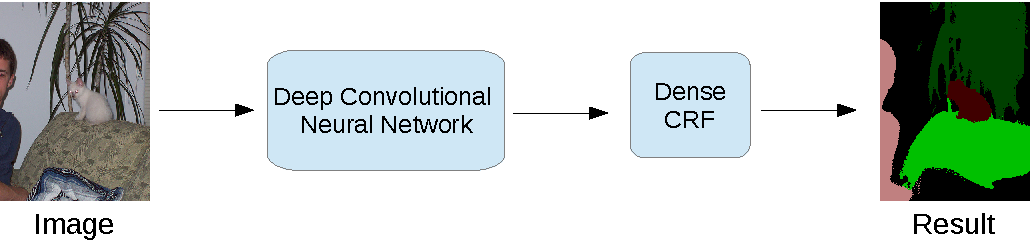
\includegraphics[width=0.9\linewidth]{fig/model_test.pdf} 
  \caption{Overview of the DeepLab CNN + CRF semantic segmentation model.}
  \label{fig:model_test}
\end{figure}

\subsection{Model Training on Fully Annotated Images}
\label{sec:train_pixel}

The network parameters $\theta$ are initialized from an
Imagenet-pretrained deep CNN model \citep{simonyan2014very} and
fine-tuned by stochastic gradient descent so as to minimize the
average log-loss 
\begin{equation}
  \label{eq:log_loss}
  L(\theta) = \frac{1}{N} \sum_{i = 1}^N \log P_i(l_i; \theta)
\end{equation}
between the model predictions and the pixel-wise ground truth
labels $\{l_i\}_{i = 1}^N$, as illustrated in
Figure~\ref{fig:model_train_pixel}. Similarly to
\citet{chen2014semantic}, we do not include the Dense CRF module into
the training pipeline for simplicity and speed during training.

Learning the DeepLab model on fully annotated images works very well
in practice, yielding excellent performance (66.4 \% IoU) in the
challenging PASCAL VOC 2012 image segmentation benchmark. However, the
need for such detailed annotations makes it harder to gather very
large training datasets and makes it difficult to train the model
for new domains, especially when the number of candidate labels
(\ie, the cardinality of the label set $\mathcal{L}$) is large.

\begin{figure}[htbp!]
  \centering
  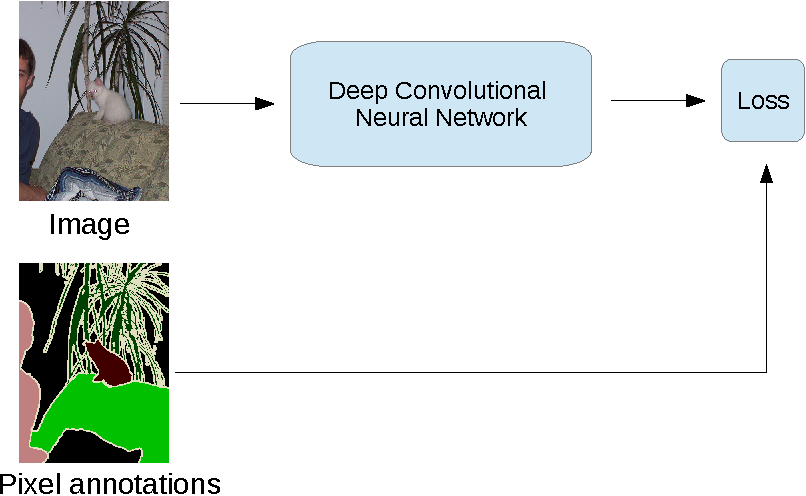
\includegraphics[width=0.9\linewidth]{fig/model_train_pixel.pdf} 
  \caption{DeepLab model training from fully annotated images.}
  \label{fig:model_train_pixel}
\end{figure}

\subsection{Model Training on Weak Bounding Box Annotated Images}
\label{sec:train_bbox}

Collecting bounding box annotations is significantly easier compared
to pixel-level ground truth segmentations. We have explored two
methods for training the DeepLab segmentation model from bounding
boxes with object-level labels. In both methods we estimate dense
segmentation maps from the bounding box annotation as a pre-processing
step, then employ the training procedure of
Section~\ref{sec:train_pixel} treating these estimated labels as
ground-truth.

The first baseline method amounts to simply considering each pixel
within the bounding box as positive example for the respective object
class. Ambiguities are resolved by assigning pixels that belong to
multiple bounding boxes to the one that has the smallest area.

\emph{GRABCUT GOES HERE}

\begin{figure}[htbp!]
  \centering
  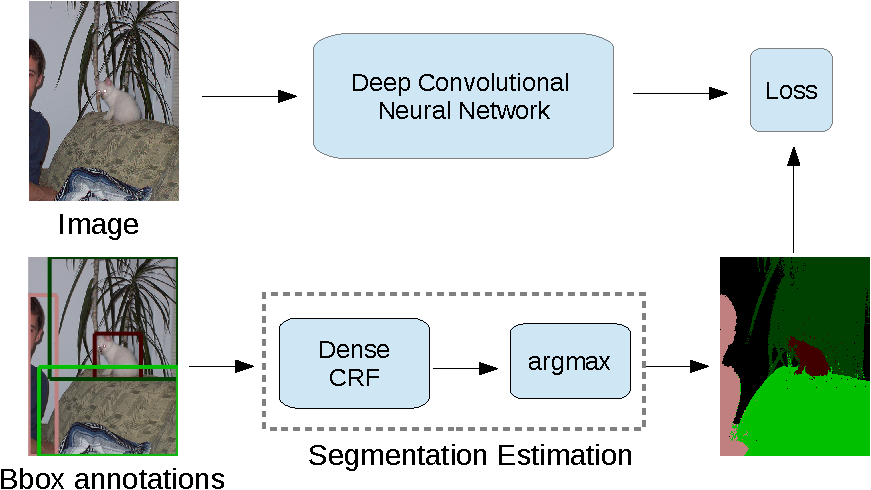
\includegraphics[width=0.9\linewidth]{fig/model_train_bbox.pdf} 
  \caption{DeepLab model training using bounding box data and
    automated foreground/ background segmentation.}
  \label{fig:model_train_bbox}
\end{figure}


\subsection{Model Training Using Weak Image-Level Labels}

Training the DeepLab segmentation model using only image-level labels
is significantly more challenging.

\paragraph{Previous MIL Approaches and their Limitations}

Previous related CNN literature employs multiple instance learning
variants to address the weak supervision problem, but has demonstrated
limited success in learning accurate segmentation models. 

In particular, recent work by \citet{pathak2014fully} attempts to
learn the CNN parameters for the segmentation model by adapting an MIL
formulation previously employed for image classification tasks
\citep{oquab2014weakly, papandreou2014untangling}. More specifically,
during training they compute an aggregate image-level response for
each class $x$ as the maximum class score across all pixel positions
$i$
\begin{equation}
  \label{eq:mil}
  \bar{f}(x; \theta) = \max_i f_i(x; \theta) \,
  \quad \mathrm{and} \quad
  \bar{P}(x; \theta) \propto \exp \left( \bar{f}(x; \theta) \right)
\end{equation}
which is then combined with the image-level ground-truth label $l$ to
compute the whole-image loss $\bar{L}(\theta) = \log \bar{P}(l;
\theta)$.

There are several limitations to this MIL-based approach to the image
segmentation problem. \emph{First}, the model does not explicitly
encourage good localization during training, since it suffices to give
strong response for the correct class anywhere within the
image. \emph{Second}, this MIL formulation does not promote good
object coverage. For example, it is often sufficient to learn a good
face detector to reliably determine whether an image contains a
person. However, this face detector will give low false-negative
responses on the rest of the human body and is thus not appropriate
for segmenting whole persons. \emph{Third}, network back-propagation
only activates a single path per label through the maximally
responding pixel position ignoring a large portion of the image
content, thus slowing down training. These issues have severely
undermined the success of previous CNN/MIL approaches to image
segmentation and the performance of such models trained on weak labels
significantly lags their counterparts trained on pixel-level
annotations, as explained in Section~\ref{sec:experiments}.

\paragraph{Adapting Expectation-Maximization for Weakly-Labeled Training}

We propose an alternative training procedure based on a modified
Expectation-Maximization (EM) algorithm adapted to our weakly-labeled
image segmentation setting.

In this setting, we consider the pixel-level semantic labels
$\{l_i\}_{i=1}^N$ as latent variables. We incorporate the image-level
semantic labels as side-information that biases the E-step of the EM
algorithm, as detailed in Algorithm~\ref{algo:em_fixed_bias} and
illustrated in Figure~\ref{fig:model_train_image}. The positive
foreground and background biases $c_f$ and $c_b$ favor the score maps
corresponding to labels present in the image according to the
image-level weak annotation. We have obtained better results by
choosing $c_f > c_b$, slightly favoring foreground objects over the
background.

\begin{algorithm}[!htbp]
  \centering
  \begin{algorithmic}[1]
    \algrenewcommand\algorithmicrequire{\textbf{Input:}}
    \Require CNN parameters $\theta$ and biases $c_f, c_b > 0$.
    \algrenewcommand\algorithmicrequire{\textbf{E-Step:}}
    \Require For each image position $i$
    \State $\hat{f}_i (x; \theta) = f_i(x; \theta) + c_f$, if label $x$ present \Comment{FG bias}
    \State $\hat{f}_i (x; \theta) = f_i(x; \theta) + c_b$, if $x$ is BG label \Comment{BG bias}
    \State $\hat{f}_i (x; \theta) = f_i(x; \theta)$, if label $x$ not present
    \State $\hat{l}_i = \argmax_i \hat{f}_i (x; \theta)$ \Comment{Hard assignments}
    \algrenewcommand\algorithmicrequire{\textbf{M-Step:}}
    \Require
    \State $\hat{L}(\theta) = \frac{1}{N} \sum_{i = 1}^N \log P_i(\hat{l}_i; \theta)$ \Comment{Expected loss}
    \State Update $\theta$ by SGD with momentum on $\hat{L}(\theta)$
    \end{algorithmic}
  \caption{Weakly-Supervised EM (fixed bias version)}
  \label{algo:em_fixed_bias}
\end{algorithm}

\begin{figure}[htbp!]
  \centering
  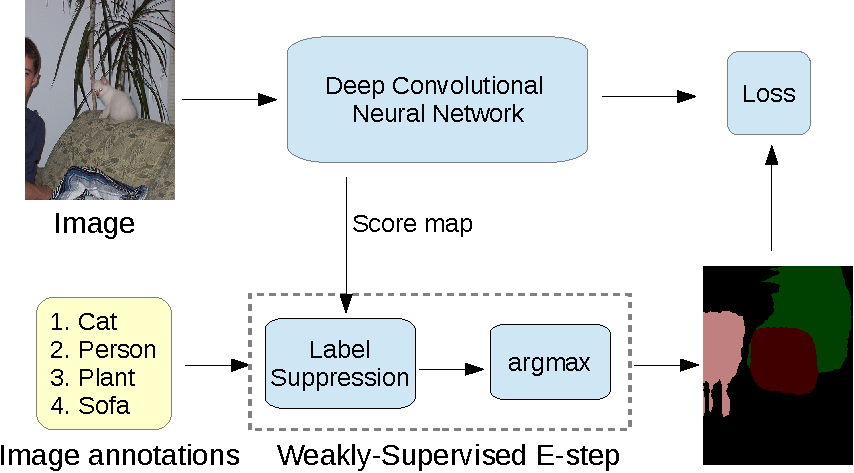
\includegraphics[width=0.9\linewidth]{fig/model_train_image.pdf} 
  \caption{DeepLab model training using image-level labels by
    biased Expectation-Maximization.}
  \label{fig:model_train_image}
\end{figure}

We have also experimented with an adaptive variant of
Algorithm~\ref{algo:em_fixed_bias} in which the biases are chosen
adaptively per image so as a pre-defined proportion of the image area
is assigned to the foreground object class. This acts as a hard
constraint that explicitly prevents the background score from
prevailing in the whole image. As reported in the experimental
section, we have found this adaptive variant to perform better in the
purely weakly supervised scenario, whereas the fixed bias variant
works best in the presense of both weak and strong annotations
discussed next.

\subsection{Model Training with a Combination of Fully and Weakly Annotated Images}

In engineering practice, we often have access to a large number of
weakly image-level annotated images and can only afford to procure
detailed pixel-level annotations for a small fraction of these
images. We propose to handle this hybrid training scenario by
combining the methods presented in the previous sections, as
illustrated in Figure~\ref{fig:model_illustrations_twoEnd}. In SGD
training of our deep CNN models, we bundle to each mini-batch a fixed
proportion of strongly/ weakly annotated images, and employ our
fixed-bias EM algorithm in estimating at each iteration the latent
semantic segmentations for the weakly annotated images. We demonstrate
in Section~\ref{sec:experiments} that one needs to annotate in
detail at the pixel-level only a fraction of the dataset and use
image-level labels for the rest of it to achieve the same level of
performance with a DeepLab model trained with the whole dataset fully
annotated.

\begin{figure}[htbp!]
  \centering
  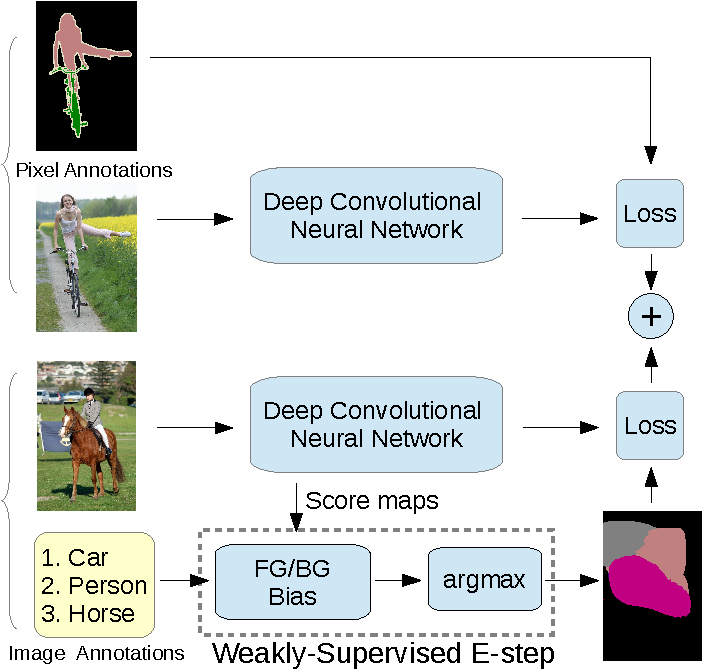
\includegraphics[width=0.9\linewidth]{fig/model_train_twoEnd.pdf} 
  \caption{DeepLab model training on a union of full (strong labels) 
    and image-level (weak labels) annotations.}
  \label{fig:model_illustrations_twoEnd}
\end{figure}

\subsection{Exploiting Annotations Across Datasets}

Finally, we discuss how we can exploit annotations across different
datasets, also allowing for the possibility annotations to be in part
weak and in part strong. For concreteness, consider also leveraging
the 81-label MS COCO dataset in learning the DeepLab model for
21-label Pascal VOC 2012 segmentation. We have experimented with the
following scenarios:
\begin{enumerate}
\item Pre-train DeepLab on MS-COCO, then replace the top-level
  classifiers weights and fine-tune on Pascal VOC 2012, using strong
  labels in both datasets.
\item Jointly train DeepLab on MS-COCO and Pascal VOC 2012 sharing
  the top-level classifier weights for the common classes, using
  strong labels in both datasets.
\item Jointly train DeepLab on MS-COCO and Pascal VOC 2012 sharing
  the top-level classifier weights for the common classes, using a
  combination of strong and weak labels.
\end{enumerare}

 %%% Local Variables:
 %%% mode: latex
 %%% TeX-master: "top.tex"
 %%% End:

\section{Experimental Evaluation}
{\bf{Dataset: }} Our model is tested on the PASCAL VOC 2012 segmentation benchmark, which includes 20 foreground object classes and one background class \citep{everingham2014pascal}. The original dataset contains $1,464$, $1,449$, and $1,456$ images for training, validation, and test, respectively. The dataset is augmented by the extra annotations provided by \citep{hariharan2011semantic}, resulting in $10,582$ training images. The performance is measured in terms of pixel intersection-over-union (IOU) averaged across the 21 classes. 

We employ VGG-16 \citep{simonyan2014very} as our DCNN, which is pre-trained on ImageNet \citep{deng2009imagenet}.


{\bf{Weighted loss: }} On the validation set. Without weighted loss: pixel accuracy $90.13\%$, mean class accuracy $73.68\%$, mean Pixel IOU $59.80\%$. With weighted loss: pixel accuracy $66.82\%$, mean class accuracy $88.81\%$, mean pixel IOU $41.77\%$.

{\bf{Incorporate Multi-Scale Features}}
mean PixelIOU $60.25\%$, after crf $64.14\%$.
\begin{figure}[ht]
  \centering
  \begin{tabular}{c c | c c | c c}
      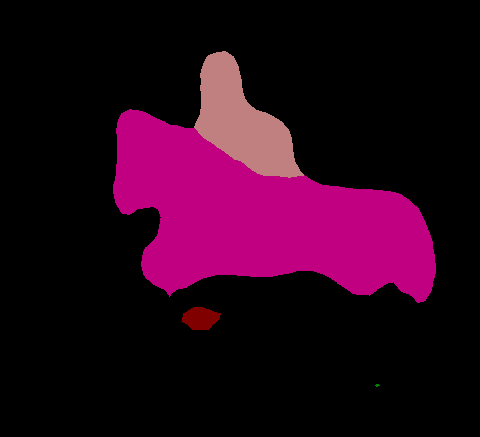
\includegraphics[height=0.12\linewidth]{fig/boundary_refine/vgg128noup_2007_000783.png} &
      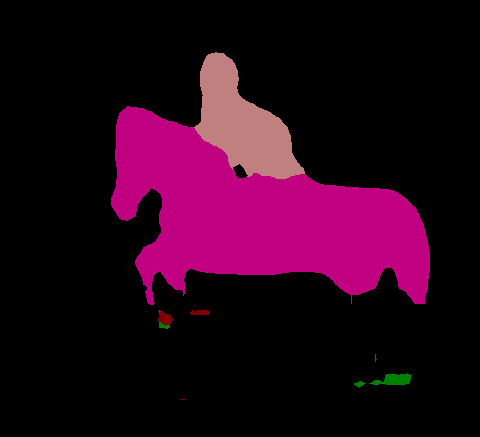
\includegraphics[height=0.12\linewidth]{fig/boundary_refine/vgg128ms_2007_000783.png} &
      
\includegraphics[height=0.12\linewidth]{fig/boundary_refine/vgg128noup_2007_001284.png} &
      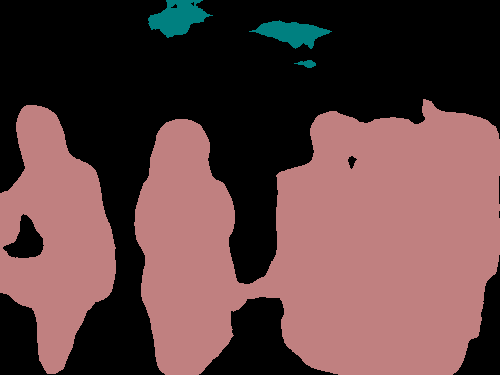
\includegraphics[height=0.12\linewidth]{fig/boundary_refine/vgg128ms_2007_001284.png} &
      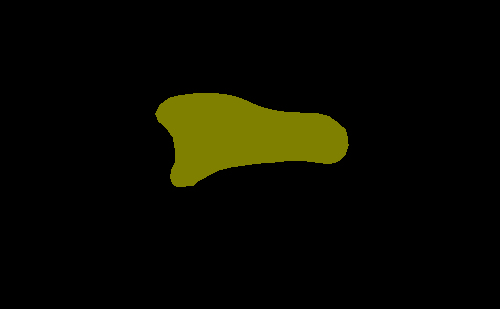
\includegraphics[height=0.12\linewidth]{fig/boundary_refine/vgg128noup_2007_001289.png} &
      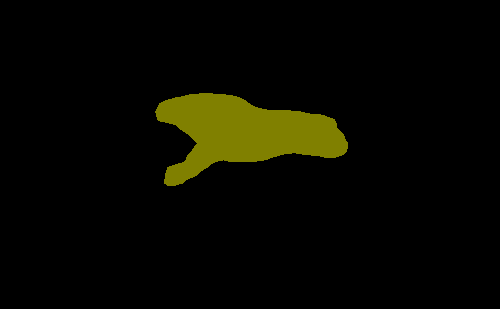
\includegraphics[height=0.12\linewidth]{fig/boundary_refine/vgg128ms_2007_001289.png} \\
      (a) & (b) & (a) & (b) & (a) & (b)
  \end{tabular}
  \label{fig:msBoundary}
  \caption{Incorporating multi-scale features improves the boundary segmentation.}
\end{figure}

{\bf{Incorporate Image-level Feature}} 
mean PixelIOU $59.86\%$, after crf $63.87\%$.

{\bf{Mean Pixel IOU along Object Boundaries: }}
To quantize the improvement of different models, we evaluate the segmention error, defined as (1 - mean IOU), around object boundaries \citep{kohli2009robust, krahenbuhl2011efficient}. Specifically, we take use of the ``void'' label annotated in PASCAL val set, which usually occurs around object boundaries. We compute the mean IOU for those pixels that are located within a narrow band (called trimap) of ``void'' labels. As shown in \figref{fig:IOUBoundary}, adding multi-scale features improve the accuracy slightly. On the other hand, refining the segmentation results by fully connected CRF significantly improve the results around object boundaries. 

\begin{figure}[ht]
  \centering
  \begin{tabular}{c c c | c c}
    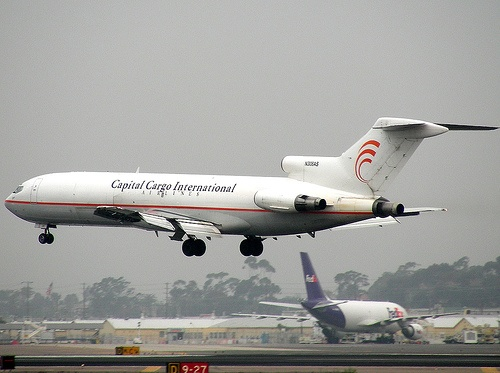
\includegraphics[height=0.12\linewidth]{fig/img/2007_002266.jpg} &
    
\includegraphics[height=0.12\linewidth]{fig/fcn8s/2007_002266.png} &
    
\includegraphics[height=0.12\linewidth]{fig/res_crf/2007_002266.png} &
    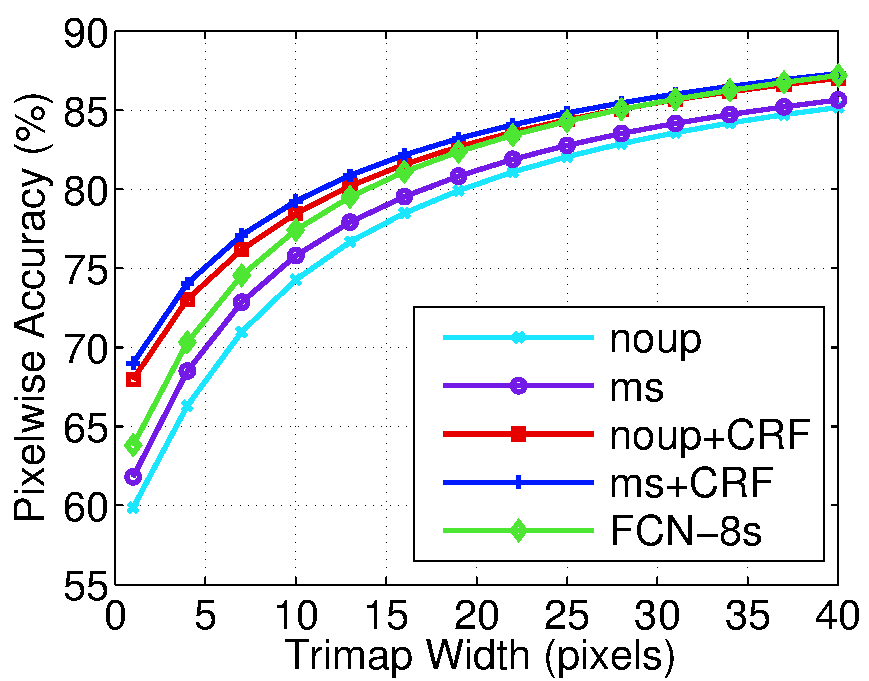
\includegraphics[height=0.12\linewidth]{fig/SegPixelAccWithinTrimap_Berkeley.pdf} &
    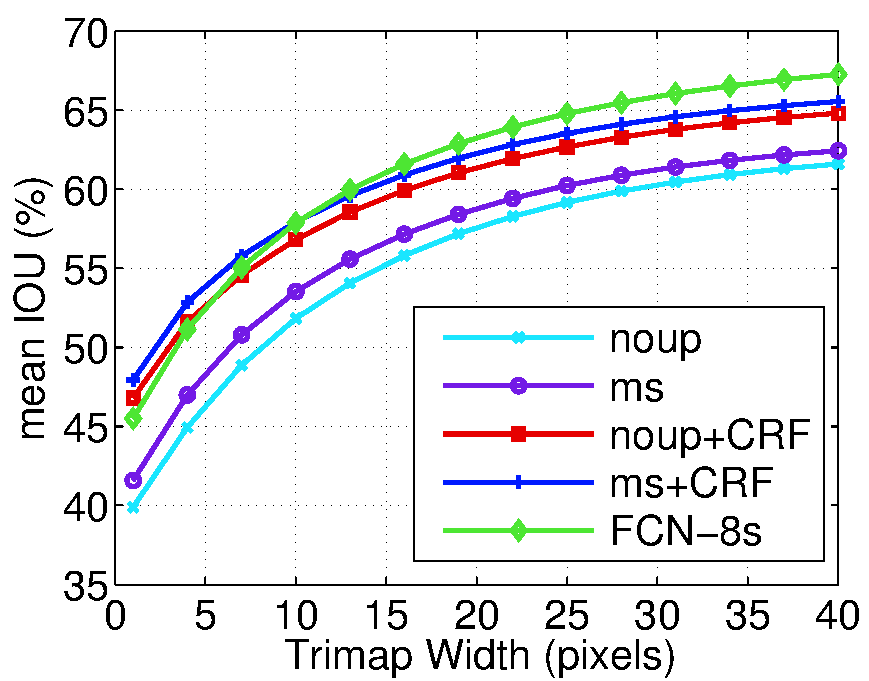
\includegraphics[height=0.12\linewidth]{fig/SegPixelIOUWithinTrimap_Berkeley.pdf} \\
    (a) & (b) & (c) & (d) & (e)
  \end{tabular}
  \caption{(Left) Some comparisons with FCN-8S: (a) image; (b) FCN-8S; (c)
    ms-crf. (d) Segmentation accuracy (pixelwise accuracy) within trimap. (e)
    Segmentation accuracy (mean IOU) within trimap. {\color{red} TODO: change
      legend. HELP: I cannot make them equally spaced....}} 
  \label{fig:IOUBoundary}
\end{figure}


\begin{figure}[!htbp]
  \centering
  %\vspace{-1.cm}
  \scalebox{0.82} {
  \begin{tabular}{c c c | c c c}
    %\addtolength{\tabcolsep}{-6.5pt}
    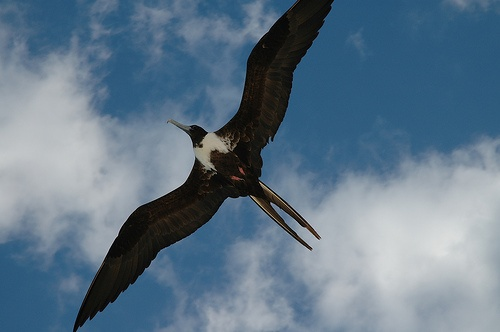
\includegraphics[height=0.12\linewidth]{fig/img/2007_002094.jpg} &
    
\includegraphics[height=0.12\linewidth]{fig/res_none/2007_002094.png} &
    
\includegraphics[height=0.12\linewidth]{fig/res_crf/2007_002094.png} &
    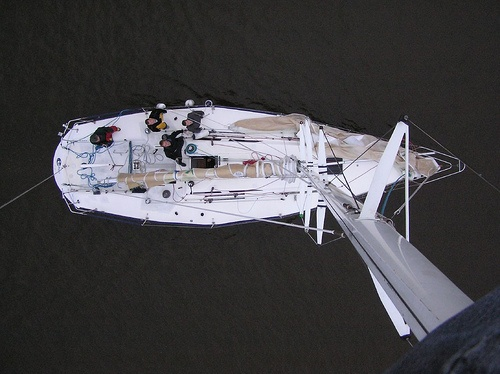
\includegraphics[height=0.12\linewidth]{fig/img/2007_002719.jpg} &
    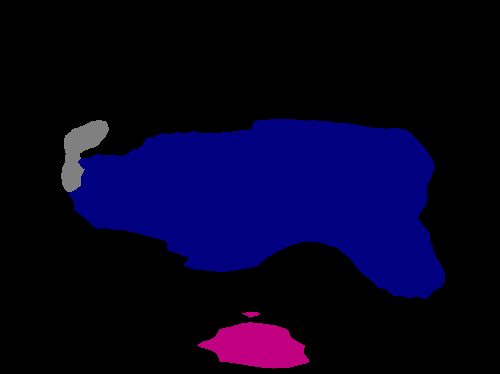
\includegraphics[height=0.12\linewidth]{fig/res_none/2007_002719.png} &
    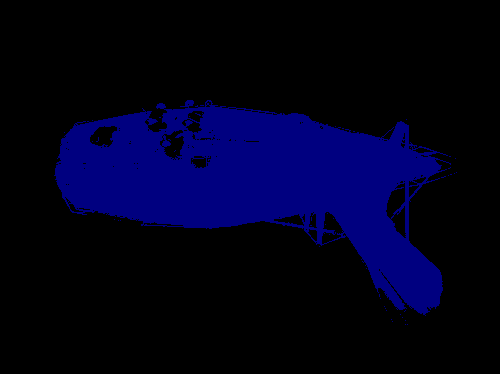
\includegraphics[height=0.12\linewidth]{fig/res_crf/2007_002719.png} \\
    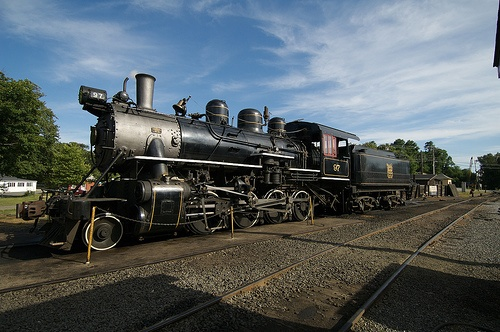
\includegraphics[height=0.12\linewidth]{fig/img/2007_003957.jpg} &
    
\includegraphics[height=0.12\linewidth]{fig/res_none/2007_003957.png} &
    
\includegraphics[height=0.12\linewidth]{fig/res_crf/2007_003957.png} &
    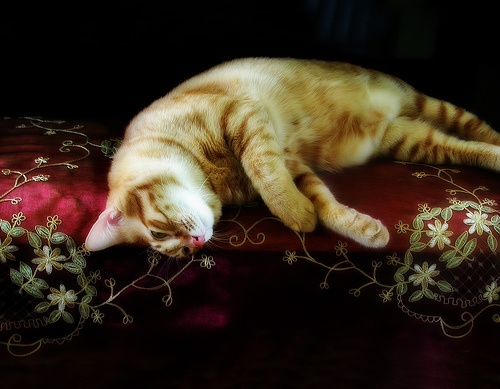
\includegraphics[height=0.12\linewidth]{fig/img/2007_003991.jpg} &
    
\includegraphics[height=0.12\linewidth]{fig/res_none/2007_003991.png} &
    
\includegraphics[height=0.12\linewidth]{fig/res_crf/2007_003991.png} \\
    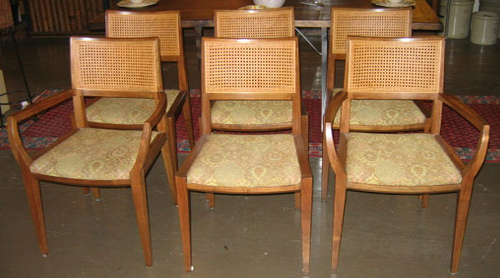
\includegraphics[height=0.10\linewidth]{fig/img/2008_001439.jpg} &
    
\includegraphics[height=0.10\linewidth]{fig/res_none/2008_001439.png} &
    
\includegraphics[height=0.10\linewidth]{fig/res_crf/2008_001439.png} &
    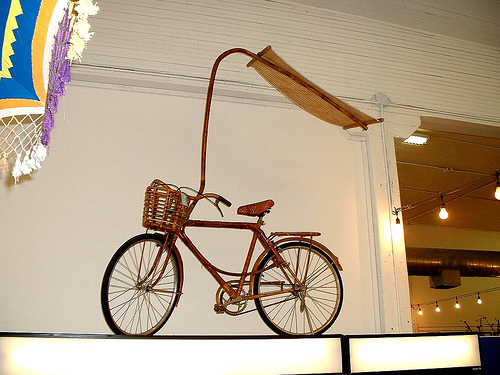
\includegraphics[height=0.12\linewidth]{fig/img/2008_004363.jpg} &
    
\includegraphics[height=0.12\linewidth]{fig/res_none/2008_004363.png} &
    
\includegraphics[height=0.12\linewidth]{fig/res_crf/2008_004363.png} \\
    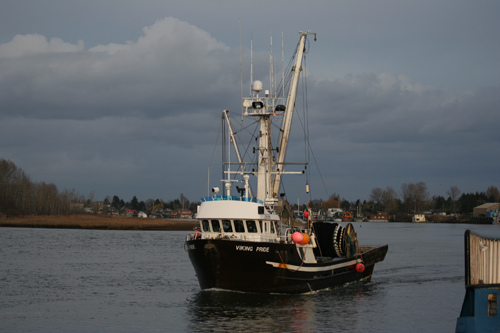
\includegraphics[height=0.12\linewidth]{fig/img/2008_006229.jpg} &
    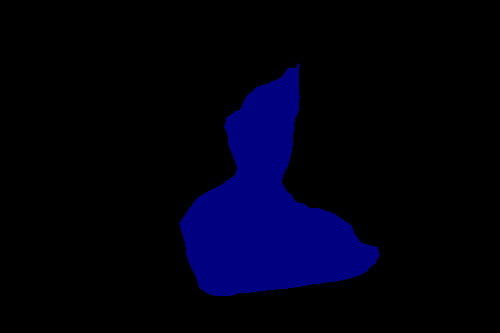
\includegraphics[height=0.12\linewidth]{fig/res_none/2008_006229.png} &
    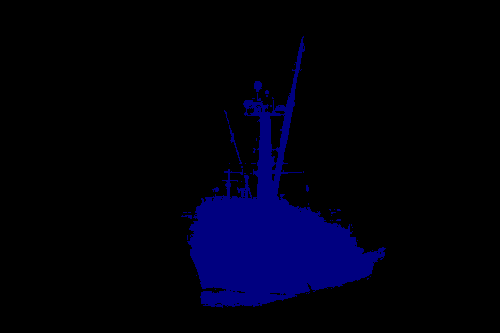
\includegraphics[height=0.12\linewidth]{fig/res_crf/2008_006229.png} &
    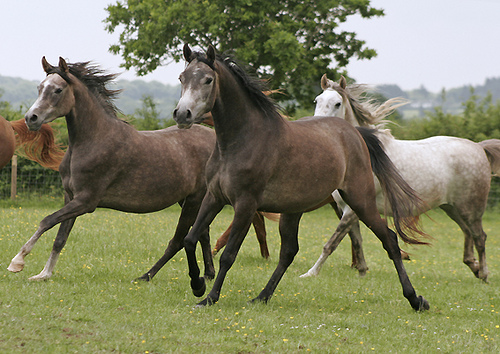
\includegraphics[height=0.12\linewidth]{fig/img/2009_000412.jpg} &
    
\includegraphics[height=0.12\linewidth]{fig/res_none/2009_000412.png} &
    
\includegraphics[height=0.12\linewidth]{fig/res_crf/2009_000412.png} \\
    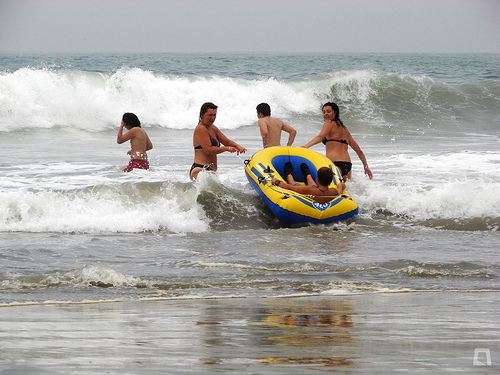
\includegraphics[height=0.12\linewidth]{fig/img/2009_000421.jpg} &
    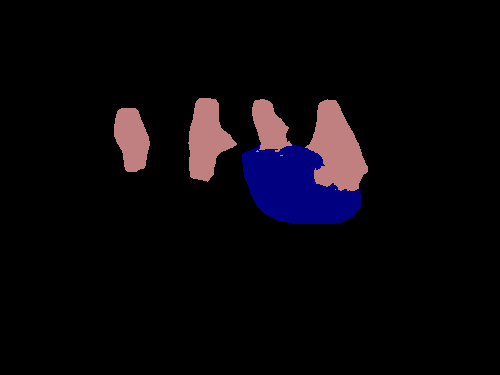
\includegraphics[height=0.12\linewidth]{fig/res_none/2009_000421.png} &
    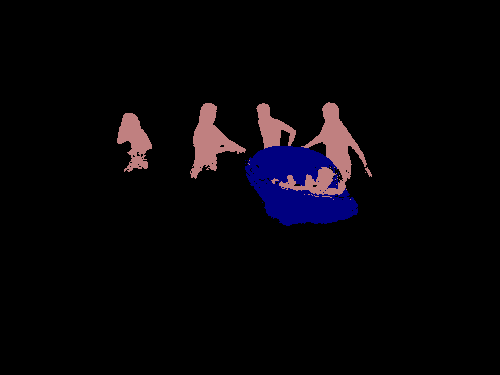
\includegraphics[height=0.12\linewidth]{fig/res_crf/2009_000421.png} &
    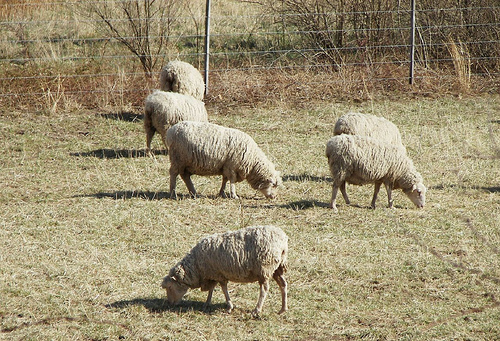
\includegraphics[height=0.12\linewidth]{fig/img/2010_001079.jpg} &
    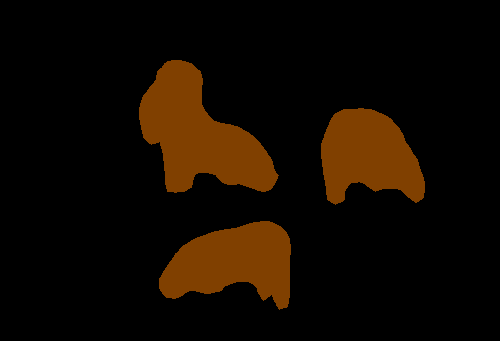
\includegraphics[height=0.12\linewidth]{fig/res_none/2010_001079.png} &
    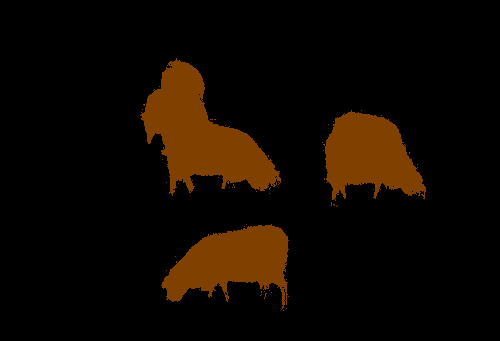
\includegraphics[height=0.12\linewidth]{fig/res_crf/2010_001079.png} \\
    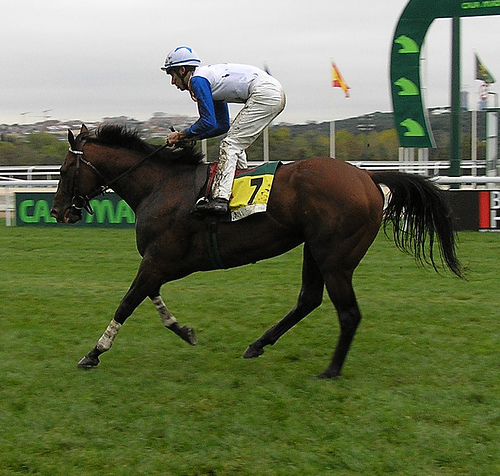
\includegraphics[height=0.12\linewidth]{fig/img/2010_000038.jpg} &
    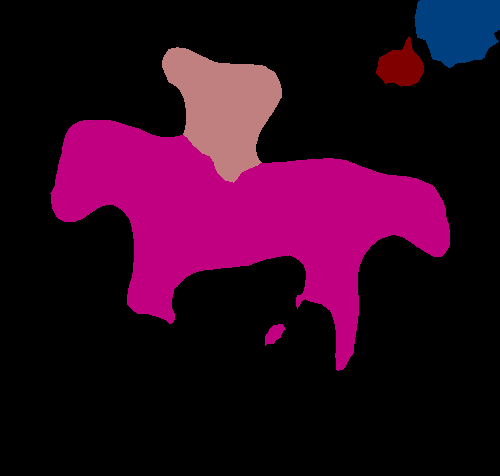
\includegraphics[height=0.12\linewidth]{fig/res_none/2010_000038.png} &
    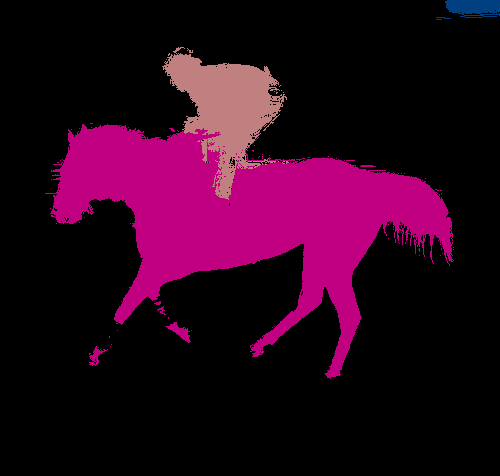
\includegraphics[height=0.12\linewidth]{fig/res_crf/2010_000038.png} &
    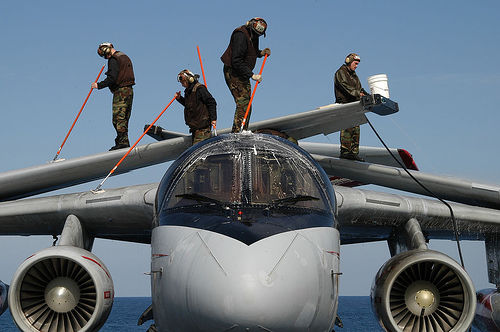
\includegraphics[height=0.12\linewidth]{fig/img/2010_001024.jpg} &
    \includegraphics[height=0.12\linewidth]{fig/res_none/2010_001024.png} &
    \includegraphics[height=0.12\linewidth]{fig/res_crf/2010_001024.png} \\
    \includegraphics[height=0.24\linewidth]{fig/img/2007_005331.jpg} &
    \includegraphics[height=0.24\linewidth]{fig/res_none/2007_005331.png} &
    \includegraphics[height=0.24\linewidth]{fig/res_crf/2007_005331.png} &
    \includegraphics[height=0.24\linewidth]{fig/img/2008_004654.jpg} &
    \includegraphics[height=0.24\linewidth]{fig/res_none/2008_004654.png} &
    \includegraphics[height=0.24\linewidth]{fig/res_crf/2008_004654.png} \\
    \includegraphics[height=0.24\linewidth]{fig/img/2007_000129.jpg} &
    \includegraphics[height=0.24\linewidth]{fig/res_none/2007_000129.png} &
    \includegraphics[height=0.24\linewidth]{fig/res_crf/2007_000129.png} &
    \includegraphics[height=0.24\linewidth]{fig/img/2007_002619.jpg} &
    \includegraphics[height=0.24\linewidth]{fig/res_none/2007_002619.png} &
    \includegraphics[height=0.24\linewidth]{fig/res_crf/2007_002619.png} \\
    \includegraphics[height=0.12\linewidth]{fig/img/2007_002852.jpg} &
    \includegraphics[height=0.12\linewidth]{fig/res_none/2007_002852.png} &
    \includegraphics[height=0.12\linewidth]{fig/res_crf/2007_002852.png} &
    \includegraphics[height=0.12\linewidth]{fig/img/2010_001069.jpg} &
    \includegraphics[height=0.12\linewidth]{fig/res_none/2010_001069.png} &
    \includegraphics[height=0.12\linewidth]{fig/res_crf/2010_001069.png} \\
    \hline
    \hline
    \includegraphics[height=0.12\linewidth]{fig/img/2007_000491.jpg} &
    \includegraphics[height=0.12\linewidth]{fig/res_none/2007_000491.png} &
    \includegraphics[height=0.12\linewidth]{fig/res_crf/2007_000491.png} &
    \includegraphics[height=0.12\linewidth]{fig/img/2007_000529.jpg} &
    \includegraphics[height=0.12\linewidth]{fig/res_none/2007_000529.png} &
    \includegraphics[height=0.12\linewidth]{fig/res_crf/2007_000529.png} \\
    \includegraphics[height=0.12\linewidth]{fig/img/2007_000559.jpg} &
    \includegraphics[height=0.12\linewidth]{fig/res_none/2007_000559.png} &
    \includegraphics[height=0.12\linewidth]{fig/res_crf/2007_000559.png} &
    \includegraphics[height=0.12\linewidth]{fig/img/2007_000663.jpg} &
    \includegraphics[height=0.12\linewidth]{fig/res_none/2007_000663.png} &
    \includegraphics[height=0.12\linewidth]{fig/res_crf/2007_000663.png} \\    
  \end{tabular}
  }
  %\vspace{-0.3cm}
  \caption{Visualization results on VOC 2012 val. For each row, we show image, segmentation result by CNN, and refined segmentation result by Fully Connected CRF. We show our failure modes in teh last two rows.} 
  \label{fig:ValResults}
\end{figure}

\section{Discussion}
\label{sec:discussion}

Our work combines ideas from deep convolutional neural networks and
fully-connected conditional random fields, yielding a novel method able to
produce semantically accurate predictions and detailed segmentation maps,
while being computationally efficient. Our experimental results show that the
proposed method significantly advances the state-of-art in the challenging
PASCAL VOC semantic image labeling task.

There are multiple aspects in our model that we intend to refine, with the most important being the 
full integration of its two main components (CNN and CRF) and training the whole
system in an end-to-end fashion.  In particular, we currently use a very naive form of piecewise training, which consists in first training the DCNN classifier, and then training the CRF while keeping the DCNN classifier fixed. But in principle the gradient of the CRF loss function can be back-propagated to the DCNN, while in recent work \citet{chen2014learning} we have exploired ways of efficiently blending inference and learning to jointly train DCNNs and CRFs. We intend to further pursue this direction in our future work. 
We also plan to experiment with more datasets
and apply our method to other sources of data such as depth maps or videos.

At a higher level, our work lies in the intersection of convolutional neural
networks and probabilistic graphical models. We plan to further investigate
the interplay of these two powerful classes of methods and explore their
synergistic potential for solving challenging computer vision tasks.



%%%%%%%%%%%%
\bibliography{egbib}
\bibliographystyle{iclr2015}

\end{document}
